\chapter{Matrix Decomposition}
\label{matrix_decomposition}
In this section I will present the algorithm, and different implementation for each framework.
\section{LU Decomposition}
A non-singular matrix $A \in \mathbb{R}^{n \times n}$ is factorized into a product of lower and upper triangular matrices $L \in \mathbb{R}^{n \times n}$ and $U \in \mathbb{R}^{n \times n}$ respectively such that $A = LU$.

LU factorization can be computed by Gaussian elimination as
shown in algorithm~\ref{alg:gaussian_elimination}, where U and L overwrites A:

\begin{algorithm}
\begin{algorithmic}
\For{$i \in  \{1 \dots n\}$}
	\For{$j \in  \{i+1 \dots n\}$}
		\State $A[j][i] = A[j][i] / A[i][i]$ \Comment{Compute L and store in A}
	\EndFor
	\For{$j \in  \{i+1 \dots n\}$}
		\For{$k \in  \{i+1 \dots n\}$}
			\State $A[j][k] = A[j][i] \times A[i][k]$ \Comment{Compute U and store in A}
		\EndFor	
	\EndFor
\EndFor
\end{algorithmic}
\caption{Gaussian elimination}
\label{alg:gaussian_elimination}
\end{algorithm}

The algorithm therefore prescribes that the data dependency flows from left to right - in other words, the matrix columns to the right depend on the columns to the left. 

\begin{figure}[H]
\centering
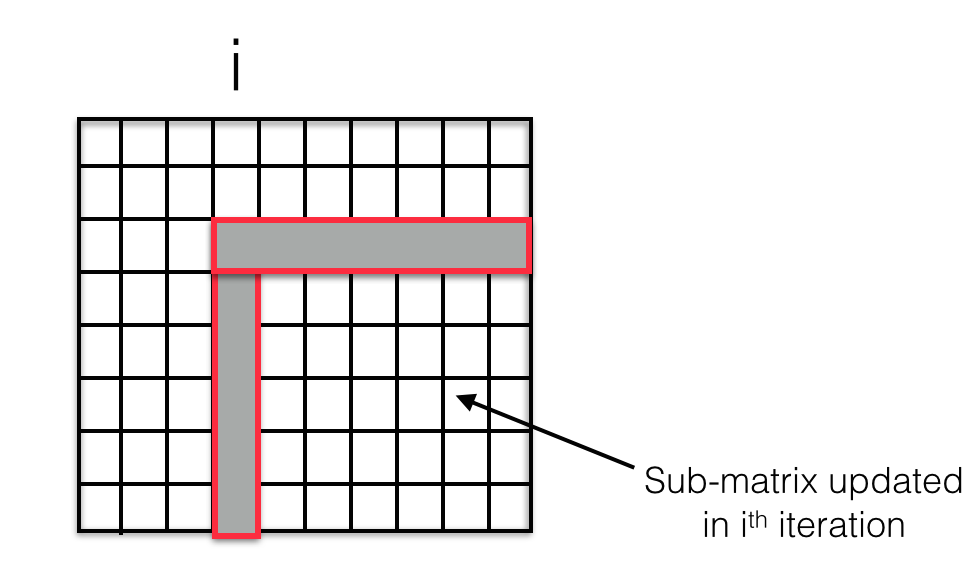
\includegraphics[width=0.5\textwidth]{LU_iteration.png}
\caption{$i$-th iteration of Gaussian elimination}
\end{figure}


This version doesn't perform pivoting. Pivoting for LU factorization is the process of systematically selecting pivots for Gaussian elimination
during the LU factorization of a matrix. This guarantees that the elimination process goes to completion, ensuring that there is a nonzero pivot at every step of the elimination process. The pivoting is not necessary if the matrix is positive semi-definite. So our test matrices will have this property.


\section{OpenMP}
OpenMP is an Application Program Interface (API) that provides a portable, scalable model for developing shared memory parallel applications.

The implementation of the LU decmposition using OpenMP (OMP) is very similar to the sequential one, the only difference consists in the OMP directives that allows the code to become parallel.

\begin{algorithm}
\begin{algorithmic}
\For{$i \in  \{1 \dots n\}$}
	\State \#pragma omp parallel for shared(A,n,i)
	\For{$j \in  \{i+1 \dots n\}$}
		\State $A[j][i] = A[j][i] / A[i][i]$ \Comment{Compute L and store in A}
	\EndFor
	\State \#pragma omp parallel for shared(A,n,i)
	\For{$j \in  \{i+1 \dots n\}$}
		\For{$k \in  \{i+1 \dots n\}$}
			\State $A[j][k] = A[j][i] \times A[i][k]$ \Comment{Compute U and store in A}
		\EndFor	
	\EndFor
\EndFor
\end{algorithmic}
\caption{Gaussian elimination}
\label{alg:omp_code}
\end{algorithm}

This compiler directive ``\textit{\#pragma omp parallel for shared(A,n,i)}" tells the compiler to auto-parallelize the for loop with OpenMP. This directive splits each \textit{for} loop iteration to a different thread, so the final submatrix elements will be computed by different threads (Note - the for loop is parallel on $j$ but not on $k$, even if the element is computed by a different thread), depending on the scheduling. In Figure~\ref{img:omp_computation_division}


\begin{figure}[H]
\centering
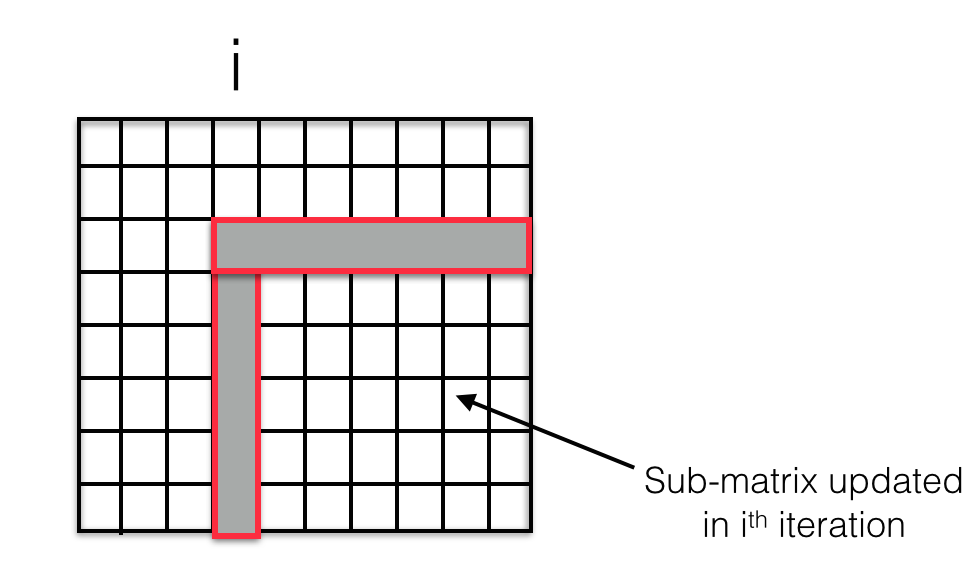
\includegraphics[width=0.5\textwidth]{LU_iteration.png}
\caption{Workload division using OpenMP}
\end{figure}



\section{MPI}
\section{CUDA}